\chapter{Herramientas utilizadas} \label{chap:herramientasutilizadas}
En este capítulo vamos a ver los orígenes de OpenStack, de donde viene y como podemos contribuir con el proyecto. 

Después discutiremos el rol de la \textit{OpenStack Foundation} y cómo los diferentes grupos de OpenStack Foundation están trabajando juntos para hacer de OpenStack la solución en la nube más importante de nuestros días. 

Además veremos una descripción general de alto nivel de OpenStack y estudiaremos como usar OpenStack para hacer que la administración de la infraestructura de IT sea más flexible. 

Para ello, iremos tratando los diferentes proyectos de OpenStack que forman el núcleo de proyectos principales, como son Nova, Neutron, Glance o Cinder entre otros. 

Listaremos también otros proyectos y servicios importantes de OpenStack haciendo énfasis finalmente en aquellos relevantes para la orquestación de NFVs y la consecución de nuestros objetivos.

\section{Orígenes de OpenStack}
OpenStack comenzó en 2010, como un proyecto conjunto de \textit{Rackspace Hosting} y \textit{NASA (National Aeronautics and Space Administration)}. La NASA contribuyó con su plataforma \textit{Nebula}, que luego se convirtió en \textit{Nova}. Rackspace contribuyó con su plataforma \textit{Cloud Files}, que más tarde acabó derivando en  en \textit{Swift}.

En abril de 2011, se produjo el lanzamiento de \textit{OpenStack Bexar} en Ubuntu. Más tarde ese mismo año, Debian incluyó \textit{OpenStack Cactus} en su distribución. En 2012, Red Hat anunció una vista previa de su distribución OpenStack también. Desde entonces, muchos otros le siguieron, incluyendo Oracle, HP y Vmware.

\section{OpenStack Foundation}
\textit{The OpenStack Foundation}, es una fundación que promueve el desarrollo global, la distribución y la adopción del sistema en la nube, proporcionando recursos compartidos para hacer crecer la nube de OpenStack. También permite a los proveedores de tecnología y desarrolladores ayudar en la producción de software en la nube. \cite{noauthor_foundation_nodate}

Existen dentro del gran número de de empresas que conforman la \textit{OpenStack Foundation} distintos estatus según el tipo de rol que tengan como miembros. Dependiendo del rol pueden tener una participación mayor o menor en el abastecimiento de fondos para capacitar y promover la comunidad y el software de OpenStack además de encargarse de la gestión del proyecto. Entre las empresas que participan se encuentran Intel, Huawei, Rasckpace, RedHat, SUSE, Mirantis, Cisco, Citrix, Lenovo, Juniper y un sin fin de compañías más.\cite{noauthor_companies_nodate}


\section{El Core de los proyectos en Openstack}
OpenStack incluye numerosos proyectos, cada uno de ellos con un estado de adopción diferente. Al mismo tiempo, se están agregando nuevos proyectos de forma regular.
Si deseamos aprender acerca de OpenStack, es importante familiarizarse con los diferentes productos que existen. Dos veces al año, la \textit{OpenStack Summit} toma  decisiones sobre la implantación de nuevos proyectos, por lo que se están agregando nuevos proyectos de forma regular.

En el sitio web de OpenStack \cite{noauthor_open_nodate}, se puede obtener una visión general actualizada de todos los proyectos que existen. OpenStack Foundation distingue entre servicios principales y servicios opcionales. Los servicios principales que forman el core son \textit{Nova, Neutron, Swift, Cinder, Keystone y Glance}. Una de las cosas interesantes que podemos ver en la web, es la adopción actual. Así, por ejemplo, vemos como Nova es una parte esencial de OpenStack, porque el 93\% de todas las nubes OpenStack lo usan.


También podemos ver que hay servicios opcionales, y algunos de ellos bastante usados en los despliegues de OpenStack, como es el caso de \textit{Horizon}, por ejemplo, que existe desde hace 7 años y lo adoptan el 86\% de todas las implementaciones de OpenStack. Pero también surgen constantemente nuevos servicios como \textit{Magnum} y \textit{Congress}. Por tanto, para cualquier servicio, si vemos los detalles de ellos, podremos ver información sobre los mismos en la wiki del proyecto, indicadores de uso, puntuación, o si es un proyecto que está comenzando o ya maduro.

\begin{figure}
    \centering
    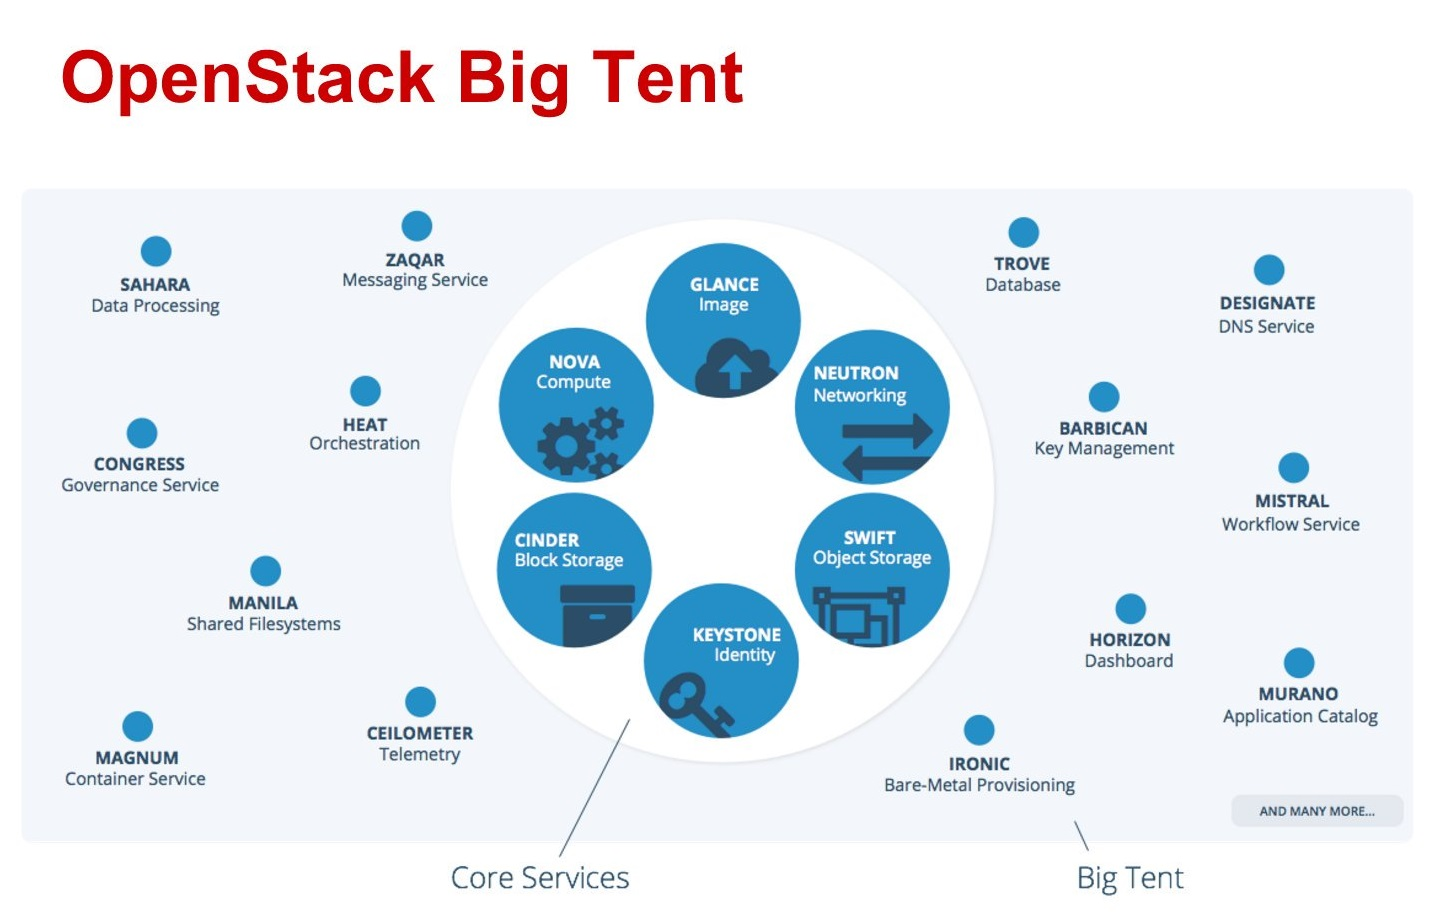
\includegraphics[width=0.7\textwidth]{imagenes/capitulo4/bigtent.png}
    \caption{Big Tent and Core Services.}
	\vspace{0.3cm}
    \footnotesize{Fuente: OpenStack}
    \label{fig:bigtent}
\end{figure}


Actualmente existen una serie de servicios dentro de OpenStack conocidos como \textit{Big Tent and Core Services} que podemos ver en la Fig.\ref{fig:bigtent} entre los que se encuentran el núcleo de servicios de Openstack antes citados, y otros servicios que son habituales encontrar en los despliegues de OpenStack y que varían en función del uso que se le vaya a dar a la infraestructura. 

Estos servicios junto a otros relevantes se describen en los siguientes apartados. Además en el anexo \ref{chap:arquitectura} podemos ver el esquema lógico de OpenStack con los componentes y relación que existe  entre la mayoría de proyectos que trataremos.

\subsection{Núcleo de servicios}

\begin{tcolorbox}[colback=orange!5!white,colframe=orange!75!black]
Jorge: Si no me equivoco, las SDN dadas por Nova son para crear las redes entre máquinas virtuales y hacia el exterior, ¿verdad? Coméntalo, porque, tal como lo pones ahora, da la sensación de que OpenStack también sirva para implementar redes SDN, y esa no es su función.
\end{tcolorbox}

\begin{itemize}
\item \textbf{Nova Compute}. Es la interfaz para el hipervisor. Se asegura de que las máquinas virtuales se puedan ejecutar en algún lugar de la nube.
\end{itemize}

\begin{itemize}
\item \textbf{Neutron Networking}. Proporciona redes definidas por software (\textit{Software Defined Networks}, SDN) en la nube a través del uso de switches software \textit{Open vSwitch}.
\end{itemize}
%Neutron es un proyecto de OpenStack usado para proporcionar conectividad de red como un servicio.

\begin{itemize}
\item \textbf{Swift Object Storage}. Con Swift podemos usar el almacenamiento en la nube de una forma inteligente, un almacenamiento que no esté vinculado a dispositivos físicos, sino que se organice en objetos binarios que se pueden dispersar por toda la nube de una manera distribuida y replicada.
\end{itemize}

\begin{itemize}
\item \textbf{Cinder Block Storage}. Como administradores, podemos usarla para proporcionar almacenamiento persistente a la máquina virtual que estamos implementando en la nube.
\end{itemize}

\begin{itemize}
\item\textbf{Keystone Identity}. Keystone nos permite combinar todo lo anterior. Podemos crear usuarios, roles o perfiles y servicios. Con esta herramienta definiremos que usuario tiene acceso a qué servicio específico y cómo los servicios específicos pueden comunicarse entre sí.
\end{itemize}

\begin{itemize}
\item \textbf{Glance Image}. Es el servicio de imágenes, necesario para implementar una instancia de una imagen en la nube. 
\end{itemize}

\subsection{Nova}
Nova es quizás el proyecto principal más importante en OpenStack \cite{noauthor_nova_nodate}. Este proyecto es el responsable de administrar el ciclo de vida de las instancias de cómputo. Ahora bien, ¿qué es una instancia de cómputo? El término de cómputo del inglés \textit{compute} es simplemente otro nombre para Nova, que podrá ser cualquier equipo o servidor en el que esté instalado el servicio y una instancia es una máquina virtual, por tanto, Nova se encarga de ejecutar la máquina virtual. 

Para ello, Nova se conecta al hipervisor pero no es el hipervisor en sí mismo. Esto lo hace muy interesante ya que independientemente del hipervisor que se esté ejecutando, bien sea Xen, KVM, VMware, vSphere o cualquier otro, Nova lo puede tratar. 
Nova instalará un agente en el hipervisor para asegurarse de que sea compatible con nuestro entorno OpenStack y se hará responsable de crear, planificar y  desmantelar las máquinas virtuales bajo demanda, incluyendo los procesos del servicio Nova que se ejecutan en el controlador de la nube, así como los agentes Nova, que se ejecutan en el hipervisor.

\subsection{Neutron}\label{subsec:Neutron}
El siguiente proyecto central de OpenStack es \textit{Neutron}. Neutron posibilita la creación de redes definidas por software. Las SDN permiten a los usuarios definir su propia red para las instancias que se implementen.\cite{noauthor_neutron_nodate}

\begin{figure}
    \centering
    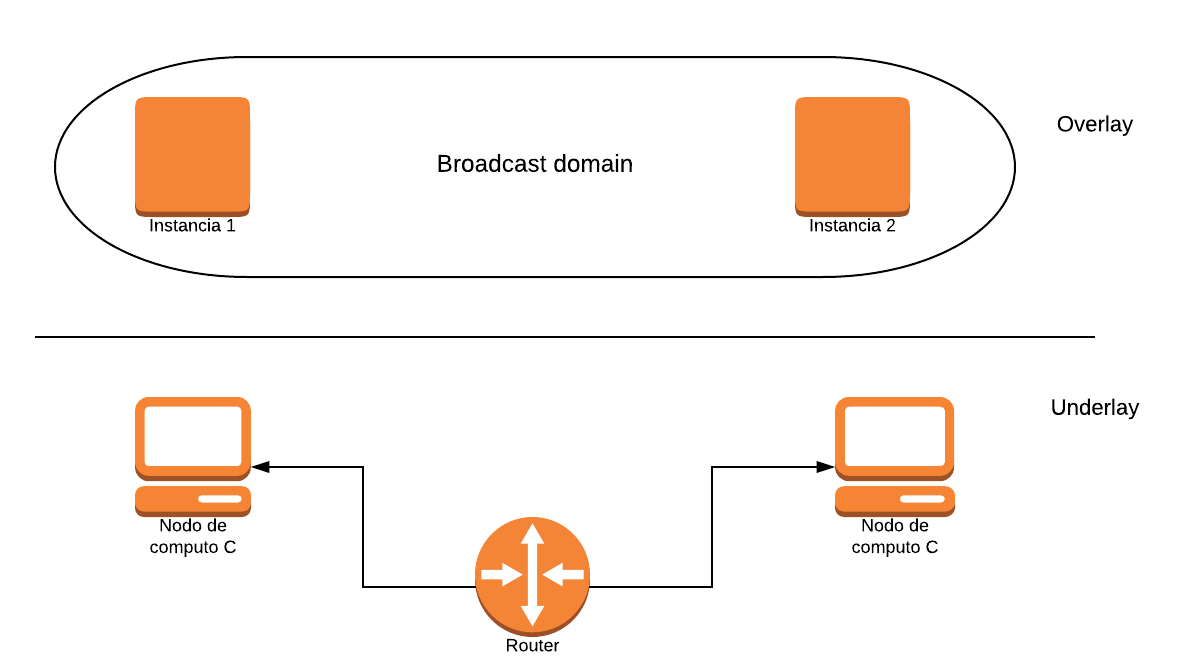
\includegraphics[width=0.7\textwidth]{imagenes/capitulo2/sdn_openstack.png}
    \caption{SDN en Openstack.}
	\vspace{0.3cm}
    \label{SDN en Openstack}
\end{figure}

Imaginemos un entorno típico de OpenStack como el de la Fig.\ref{SDN en Openstack}. En este supuesto entorno hay dos nodos C de cómputo diferentes. Estos nodos se conectarán mediante el uso de una red física que simulamos como un router en la figura. Llamamos a esta parte, la red subyacente , \textit{underlay network}. En esta red física se realizará enrutamiento y lo necesario para que funcione. Esta parte de la configuración de la red física será típicamente lo que el usuario de OpenStack no conocerá.

El nivel de usuario, que será el nivel más alto, es lo que llamaremos la red de superposición o \textit{network overlay}. En el nivel de usuario, puede haber distintas instancias ejecutándose en lugares diferentes (instancias 1 y 2 ejecutándose cada una en un nodo), pero el usuario puede desear implementar estas instancias como si se usaran en el mismo dominio de difusión (\textit{broadcast domain}), formando así una red lógica.

En un dominio de difusión, las instancias estarán en la misma red, por lo que, ¿cómo puede ser que estén en el mismo dominio de difusión si en la red subyacente tenemos diferentes redes físicas? Esto es exactamente de lo que Neutron se está ocupando mediante el uso de redes definidas por software. Para hacerlo, Neutron necesita interconectar la arquitectura de la red física, para lo cual utiliza una arquitectura conectable (\textit{pluggable architecture}). Esta arquitectura conectable admite muchos proveedores y tecnologías de redes. Por lo tanto, si se ha realizado una gran inversión en alguna tecnología de red patentada, es probable que haya un buen plugin de Neutron disponible. La mayoría de los proveedores de red tienen plugins de Neutron, por lo que no tendremos por norma general problemas con esto.

Además, Neutron proporciona una API para que los usuarios definan las redes y los archivos adjuntos en ellas. Como resultado, para un programador o administrador será relativamente sencillo crear su propio entorno de SDN, como veremos más adelante.

\subsection{Swift}
El siguiente proyecto central de OpenStack del que hablaremos es \textit{Swift}. Swift está diseñado para proporcionar escalabilidad en el nivel de almacenamiento. Funciona con objetos binarios para almacenar datos de una manera distribuida y replicada. \cite{noauthor_swift_nodate}

El almacenamiento finalmente termina en un disco duro y un disco duro es un dispositivo físico. El problema con los dispositivos físicos es que son limitados y no son muy escalables, por lo que si todo nuestro almacenamiento en la nube estuviese en un servidor que proporciona diferentes discos duros, no tendríamos escalabilidad. Para tenerla, Swift ofrece un modelo de almacenamiento basado en objetos.

\begin{figure}
    \centering
    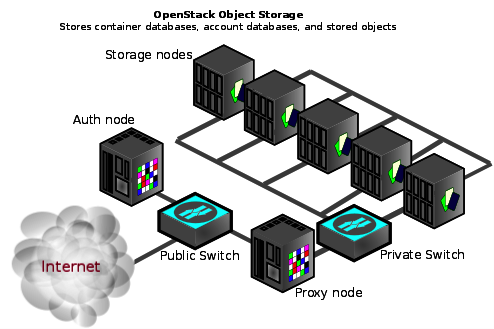
\includegraphics[width=0.7\textwidth]{imagenes/capitulo2/swift_storage.png}
    \caption{Almacenamiento de objetos distribuido con Swift.}
    \footnotesize{Fuente: Mirantis}
	\vspace{0.3cm}
    \label{Swift Storage}
\end{figure}

Para entender el funcionamiento de Swift nos fijaremos en la Fig.\ref{Swift Storage}. La idea sobre Swift es que tenemos una aplicación que usaremos para escribir datos. En un entorno OpenStack, la aplicación no escribe un archivo en el disco duro, sino que esta puede interactuar con el almacenamiento de objetos de Swift que  se está comunicando a su vez con muchos nodos de almacenamiento.

En la Fig.\ref{Swift Storage} podemos ver distintos nodos de almacenamiento (\textit{Storage nodes}). Swift está usando un proxy y cuando el proxy de Swift recibe datos de la aplicación, va a crear objetos binarios. Estos objetos binarios son los fragmentos de datos.

Digamos que tenemos objetos binarios A, B y C. En Swift, el objeto binario A se puede almacenar en uno de los nodos de almacenamiento, el objeto binario B en otro y el C en otro diferente. Si solo se almacena una vez, el sistema no será tolerante a fallos, por lo que Swift incluye un algoritmo de replicación para almacenar los objetos binarios en múltiples nodos. Por defecto, esto se hará tres veces, es decir, cada objeto se almacenará en tres nodos diferentes, aunque podríamos almacenarlo en un número mayor de nodos si así lo requerimos.

Este proceso hace que el almacenamiento sea más eficiente ya que en el momento en que la aplicación necesita recuperar los datos, se dirigirá al proxy Swift nuevamente y el proxy Swift estará utilizando un algoritmo avanzado para determinar exactamente dónde residen los objetos binarios, enviando llamadas a todos los nodos de almacenamiento involucrados. Debido a todos estos nodos de almacenamiento que podrán funcionar en paralelo, los datos llegarán al proxy de Swift, y por lo tanto, a la aplicación, de una manera muy rápida. Y así es como se consigue con OpenStack hacer que el almacenamiento sea escalable.

Aún tiene más ventajas, imaginemos que estos nodos de almacenamiento son de un terabyte cada uno. Cuando nos estamos quedando sin almacenamiento disponible, es bastante fácil agregar un par de nodos de almacenamiento Swift más, e incluso se pueden reequilibrar los objetos binarios que están escritos en la configuración de almacenamiento de Swift.

La aplicación que se usa para hablar con Swift, está utilizando una API RESTful.
REST es una forma estándar de comunicación en un entorno OpenStack como ya sabemos. Esto significa que la aplicación no está escribiendo un archivo en un sistema de archivos, sino que está utilizando una llamada RESTful API, que es entendida por Swift proxy. La API RESTful es el lenguaje nativo de OpenStack, y eso convierte a Swift en la opción nativa para el almacenamiento de objetos en OpenStack.

\subsection{Glance}
El siguiente proyecto importante de OpenStack es Glance. Glance se usa para almacenar imágenes de disco de la máquina virtual\cite{noauthor_glance_nodate}. Las máquinas virtuales, que son las instancias, no están instaladas, sino que se generan a partir de una imagen que podemos descargar\cite{noauthor_get_nodate}. Es como arrancar Linux desde un live CD. Las imágenes se pueden descargar fácilmente o se pueden crear para que coincidan con las necesidades específicas dentro de una organización.

En la web se proporcionan diferentes imágenes en la nube para diferentes sistemas operativos, que incluyen CentOS, Debian, Fedora, básicamente, todas las principales distribuciones de Linux, e incluso incluye Microsoft Windows.

Una imagen interesante es la imagen de CirrOS y lo es porque es muy pequeña, solo de trece megabytes, motivo por el cual la usaremos para realizar nuestros despliegues posteriormente debido a la limitación principalmente de RAM de nuestro entorno.

Así pues, Glance es como nuestra tienda de imágenes. Esto significa que si un administrador desea iniciar una instancia, iniciará la instancia desde el almacén de imágenes de Glance y es por ello que Glance es un pilar básico de OpenStack.

Para que todo sea escalable, el almacén de imágenes de Glance normalmente usa el almacenamiento de objetos Swift como un back-end. Por supuesto no hay porque utilizar el almacenamiento de objetos de Swift, pero usarlo lo hace más escalable. La otra opción sería usar el almacenamiento local como back-end para Glance, pero estariamos usando entonces almacenamiento local y por tanto vinculado a un servidor físico que contiene las imágenes física y que no es muy escalable.

\subsection{Cinder}
El siguiente proyecto esencial de OpenStack es Cinder\cite{noauthor_openstack_nodate-6} encargado de proporcionar almacenamiento persistente a las instancias. 

Por defecto, el almacenamiento de las instancias es efímero.  Es también como arrancar desde un live CD en Linux. Si trabajamos desde un live CD e intentamos cambiar el archivo de configuración, ¿dónde se cambiaría? porque la imagen del live CD está cargada en la RAM y realmente no existe en ningún disco duro grabable.

Este es el mismo problema que tenemos con las imágenes de Glance, y es por eso que en OpenStack, el almacenamiento instantáneo es efímero. Cinder es lo que permite a los administradores asignar almacenamiento persistente a las instancias.

Cinder también puede usar diferentes backends. Puede ser un almacenamiento local, que de forma predeterminada será LVM de Linux (\textit{Linux Volume Manager}) o puede incluir almacenamiento de objetos Swift y Ceph, incrementando así la escalabilidad.

\subsection{Keystone}
\begin{figure}
    \centering
    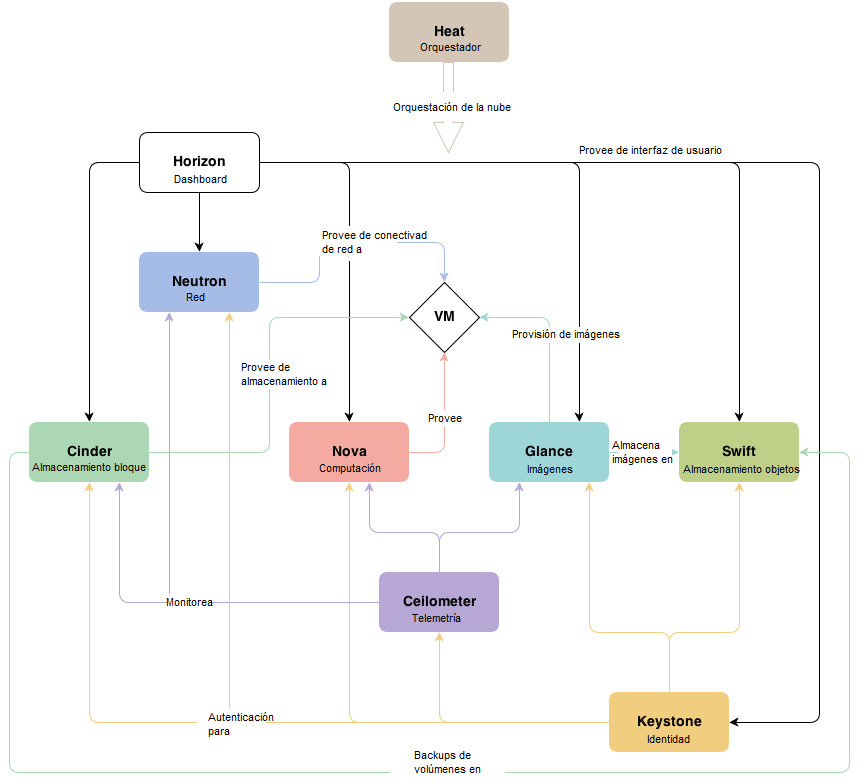
\includegraphics[width=0.7\textwidth]{imagenes/capitulo4/arquitectura1.png}
    \caption{Arquitectura conceptual de OpenStack.}
	\vspace{0.3cm}
    \footnotesize{Fuente: Daniel Romero Sanchez, “Openstack desde cero - Keystone”, DBigCloud, 2015} 
    \label{arquitecturaOpenStack}
\end{figure}

Ninguna nube OpenStack podría existir sin los servicios proporcionados por el proyecto Keystone. Keystone se usa para la autenticación, autorización y enumeración de todos los servicios y backends.\cite{noauthor_keystone_nodate}

Con servicio nos referimos en este caso a cualquiera de los proyectos que se implementa en OpenStack. De este modo, si queremos poder ejemplo acceder a Nova, Nova debe definirse como un servicio en Keystone y el backend proporciona una URL que da acceso al servicio específico. Como administradores, también podremos consultar estos servicios y backends como veremos.

Keystone es un elemento central en OpenStack tal como refleja la Fig.\ref{arquitecturaOpenStack} donde aparecen los principales proyectos de OpenStack que hemos ido enumerando y las relaciones comentadas que existen entre ellos.

En Keystone, los usuarios y roles se crean y se asignan a proyectos, que también se conocen como \textit{tenants}. Un proyecto, también conocido como tenant, por lo general, es un cliente de OpenStack. Si OpenStack se usa como una nube pública, pueden ser diferentes empresas que están contratando espacio en la nube en OpenStack y para distinguir entre los recursos disponibles para un cliente y otro cliente, OpenStack está utilizando esta noción de proyectos o tenants.

En un entorno de proyecto, normalmente se crearán cuentas de usuario a las que se asignarán roles específicos y dependiendo del rol asignado a una cuenta de usuario, los usuarios tendrán más o menos opciones para hacer cosas en OpenStack.

De todo ello se ocupa Keystone, por lo tanto, Keystone es un repositorio central para todos los servicios y resultados de backends.

De forma predeterminada, Keystone está utilizando una base de datos, que es la base de datos MariaDB (derivada de MySQL), para almacenar información, lo cual no significa que no podamos cambiarla a otras que queramos usar como OracleDB o bien, usar un directorio LDAP.

\subsection{\textit{The big tent}}
Otros proyectos interesantes de OpenStack que no forman parte de los principales pero que tienen un alto índice de adopción son:

\begin{itemize}
\item \textbf{Ceilometer.} Ceilometer es conocido como el servicio de telemetría y se usa para medición y registro. Recopila datos que pueden ser consultados por un software de terceros, pero también se pueden usar para obtener estadísticas de uso que se pueden pasar al servicio de Heat. Según la información que obtiene de Ceilometer, Heat puede ampliar o reducir automáticamente la cantidad de recursos en la nube.\cite{noauthor_celiometer_nodate}

\item\textbf{Trove.} Trove es un Database as a Service para OpenStack. Provee a OpenStack de motores de bases de datos relacionales y no relacionales. Su objetivo es ofrecer la funcionalidad de base de datos a los usuarios sin la necesidad de ocuparse de tareas de administración complejas. Como resultado, los usuarios así como los administradores pueden implementar instancias de base de datos fácilmente.\cite{noauthor_trove_nodate}

\item \textbf{Sahara.} Sahara es Big Data en OpenStack. Está configurado para ofrecer una fácil implementación de Hadoop sobre OpenStack. Sahara se ocupa de los parámetros de Hadoop, como la versión, la topología del clúster y el hardware. El usuario proporciona estos parámetros y Sahara implementará automáticamente el clúster. Sahara puede agregar y eliminar nodos fácilmente al clúster según sea necesario.\cite{noauthor_sahara_nodate}

\item \textbf{Ironic.} Ironic es el programa de aprovisionamiento  bare metal de OpenStack y fue desarrollado para implementar máquinas físicas (y no máquinas virtuales). Ironic es una API bare metal de hipervisor con un conjunto de complementos que interactúan con los hipervisores de bare metal. Utiliza PXE (\textit{Preboot Execution Enviornment}) o IPMI (\textit{Intelligent Platform Management Interface}) para aprovisionar y encender máquinas o apagarlas. Ironic también funciona con complementos específicos del proveedor para aportar funcionalidades adicionales.\cite{noauthor_ironic_nodate}


\item \textbf{Zaqar.} Zaqar es el servicio de mensajería OpenStack. Es una alternatia a una instalación independiente del servicio de mensajería AMQP (\textit{Advanced Message Queuing Protocol}) o ZeroMQ. Zaqar puede usar una API REST basada en HTTP, así como una API basada en websocket para la comunicación. Zaqar permite el manejo de colas de múltiples usuarios y proporciona una alta disponibilidad interna y escalabilidad, lo cual es un reto en los servicios de mensajería independientes.\cite{noauthor_zaqar_nodate}

\item \textbf{Manila.} Originalmente está basado en Cinder. Manila es el servicio de sistema de archivos de OpenStack. Ofrece una alternativa al almacenamiento local o de objetos, proporcionando así una solución de almacenamiento flexible.\cite{noauthor_manila_nodate}

\item \textbf{Designate.} El proyecto Designate proporciona DNS como servicio para OpenStack: acceso a API REST para administración de dominios y registros, utilizable en entorno multi-tenant, integrado con Keystone para autenticación, se integra con Noa y Neutron para la generación automática de registros DNS y soporte nativo para Bind9 y PoweDNS.\cite{noauthor_designate_nodate}

\item \textbf{Barbican.} Barbican implementa seguridad y administración de claves en la nube, proporcionando una API REST. Está diseñado para almacenamiento, aprovisionamiento y administración de todo tipo de claves, incluidas contraseñas, claves de cifrado y certificados X.509.\cite{noauthor_barbican_nodate}

\item \textbf{Magnum.} El proyecto Magnum fue desarrollado para permitir la administración de contenedores en OpenStack.  Su objetivo es integrar los motores de orquestación de contenedores como recursos de primera clase en OpenStack. Un ejemplo importante de este tipo de motor es Kubernetes: Magnum permite integrar Kubernetes en un entorno OpenStack para que pueda ejecutar contenedores orquestados de Kubernetes encima de OpenStack. El resultado es que se pueden integrar contenedores en OpenStack de manera similar a como las instancias se integran encima de Nova.\cite{noauthor_magnum_nodate}

\item \textbf{Murano.} El proyecto Murano proporciona un catálogo de aplicaciones para OpenStack. El objetivo de este proyecto es permitir que los desarrolladores de aplicaciones y los administradores de la nube publiquen las aplicaciones disponibles en un catálogo. Esto permite a los usuarios consultar una lista de aplicaciones en la nube de una manera fácil de navegar.\cite{noauthor_murano_nodate}

\item\textbf{Congress.} Congress es un proyecto de Policy as a Service. Proporciona gobernanza y cumplimiento como servicios en la nube. El administrador puede definir políticas y Congress se encargará de implementar estas políticas.\cite{noauthor_congress_nodate}

\item\textbf{Heat.}  Se usa para desplegar un conjunto de instancias en un entorno OpenStack. Esto nos permite desplegar múltiples máquinas virtuales relacionadas de una manera sencilla. Heat usa HOT (Heat Orchestration Template) o AWS CloudFormation template para definir las pilas o conjuntos de instancias orquestando de esta forma el resto de proyecto (ver Fig.\ref{arquitecturaOpenStack}). Este proyecto lo trataremos en detalle en la sección \ref{subchap:heat}.
\end{itemize}

\subsection{Detrás de los proyectos de OpenStack}
Detrás de todos estos servicios de OpenStack que forman el núcleo básico, también hay algo más. Siempre se requieren algunos servicios vitales y estos incluyen:

\begin{itemize}
\item La sincronización de tiempo o \textit{timestamp}. Esta es necesaria porque muchos servicios están utilizan timestamps para la comunicación, por ejemplo en Keystone. Keystone está enviando tickets que se basan en timestamps y si los servicios no llegan a un acuerdo en el momento adecuado, entonces, no habrá comunicación.
\item Otro servicio es la base de datos de MariaDB de la que hemos estado hablando cuando hablamos sobre Keystone, usada para almacenar toda la información relacionada con la nube. Esto es muy interesante porque como administradores, podremos consultar la base de datos y obtener información sobre lo que está sucediendo fuera de ella.
\item También está la cola de mensajes o \textit{message queue}. La cola de mensajes es un componente esencial al que los servicios acceden para intercambiar mensajes de forma ordenada entre los distintos servicios necesarios. Es como un servidor de correo SMTP en el manejo del correo electrónico, un servicio que se encarga de entregar el mensaje al destino correcto. Openstack incorpora AMQP como servicio de mensajería, siendo el agente predeterminado RabbitMQ.
\end{itemize}

En una implementación de OpenStack que está automatizada, todo esto se creará automáticamente. Si por contra optamos por implementar OpenStack manualmente, deberemos encargarnos nosotros mismos de estos tres servicios esenciales.

\section{La API RESTful}

Para comprender OpenStack, hay que entender el funcionamiento de la \textit{API RESTful}. REST es un método genérico para proporcionar acceso a todos los componentes de OpenStack. Todas las APIs de OpenStack son RESTful, lo que proporciona un acceso uniforme. Esto facilita el trabajo para los desarrolladores, ya que se usan los mismos estándares en todas partes y un desarrollador puede usar el mismo lenguaje en todo lo que hace.

El acceso a la API RESTful se puede utilizar al implementar comandos, pero también directamente usando curl, un proyecto de software consistente en una biblioteca (\textit{libcurl}) y un intérprete de comandos (\textit{curl}) orientado a la transferencia de archivos y que soporta protocolos como FTP, FTPS, HTTP, HTTPS, TFTP, SCP, SFTP, Telnet, DICT, FILE y LDAP entre otros.\cite{noauthor_curl_nodate}

Vamos a hacer una pequeña demostración de lo que la API RESTful hace posible.
Imaginemos que estamos en una máquina OpenStack. En la máquina OpenStack, podemos usar un comando como este:

\begin{lstlisting}[style=Consola]
stack@jorge-All-Series:/opt/stack# curl -s -X POST http://192.138.4.201:5000/v2.0/tokens -H "Content-Type: application/json" -d ' ("auth": {"tenantName": "'"$OS_TENANT_NAME"'", "passwordCredentials": {"username": "'"$OS_USERNAME"'", "password": "'"$OS_PASSWORD"'"}}}' | python -m json.tool
\end{lstlisting}

De este modo, estamos haciendo una llamada a la API de forma directa. Como administradores, no nos interesará hacer esto, pero es una forma de exponer lo que sucede detrás de la interfaz web de Horizon, o de la línea de comandos.

Al usar este comando, estamos accediendo a un endpoint de la API utilizando el método POST, por lo que, estamos haciendo un POST a tokens y estamos especificando en el content-type que el tipo de datos sea json, proporcionando además  credenciales de autenticación. Por último, redirigimos el resultado a Python, que está utilizando la herramienta json.

Como resultado obtendremos:

\begin{lstlisting}[style=Consola]
          ],
          "endpoints links": [],
          "name":"Image Service",
         "type":"image"
     },
          "endpoints": [
                {
                    "adminURL:"http://10.5.1.201:35357/v2.0",
                    "id":"5797558684004446bbe92448ffd3f6fw",
                    "internalURL":"http://10.5.1.201:5000/v2.0"
                    "publicURL":"http://10.5.1.201:5000/v2.0"
                    "region":"RegionOne"
                }
            ],
           "endpointss_links": [],
           "name":"keystone",
           "type":"identity"
     }
],
"token":{
    "audit_ids": [
          "3RAGfK16Ssui3kA6M2Cgmg"
      ],
     "expire":"2018-07-28T14:51:152",
     "id":"bb9ad8edda2e434a9b261c539a8bf1ea",
     "issued_at":"2018-07-28T14:51:152.86034ZZ",
     "tenant": {
           "description":"deafult tenant",
           "enabled":"true",
           "id":"7db988ced11842e3af279aaa2425f362",
           "name":"demo"
       }
},
"user": {
     "id":"ae8380b700344341994183c0cd6db4f9",
     "name":"demo",
     "roles": [
            {
                "name": "_member_"
            }
       ],	
      "roles_links": [],
      "username": "demo"
\end{lstlisting}

Esta es la información en crudo que OpenStack proporciona al administrador. Más adelante veremos la existencia de una línea de comandos que hace que esta tarea más sencilla y que existe también una interfaz web,  Horizon, que la hace mucho más amigable e intuitiva para el usuario.

Como conclusión, saber que uno de los puntos fuertes de OpenStack es que todo es compatible con la API RESTful y debido a ello cada vez es más fácil comunicarse entre los diferentes servicios.

\section{Horizon}
Al tratar la API RESTful y en la Fig.\ref{arquitecturaOpenStack} vemos un proyecto del que aún no hemos hablado, Horizon \cite{noauthor_horizon_nodate}. Horizon es el dashboard de OpenStack y proporciona una interfaz web para una fácil administración de instancias y otras propiedades de OpenStack tanto para los administradores de la nube como para los usuarios que se creen y que quieran gestionar los recursos proporcionados de dicha nube.

Horizon es uno de los componentes más populares de OpenStack. Se usa con mucha frecuencia porque es mucho más fácil de usar que la poderosa interfaz de línea de comando y esa es la razón por la cual los usuarios finales usan Horizon.

Como nota importante, al trabajar desde Horizon notaremos que la perspectiva que se obtiene como usuario administrador es diferente a la perspectiva que se verá como un usuario tenant o invitado.
El usuario administrador es responsable de la administración de los tenants así como de la infraestructura de la nube, mientras que un usuario tenant es responsable de administrar el entorno del tenant, de ahí las diferencias que se apreciarán.

\subsection{API REST vs CLI vs Horizon}
Vamos a hacer una pequeña comparativa entre la API, la línea de comandos o CLI (Command Line Interface) y Horizon. Hemos visto previamente un comando insertado con el que usamos la API. Esta API puede ser utilizada por cualquiera o cualquier aplicación puede usarla para solicitar información directamente de OpenStack y la respuesta se proporciona en el formato json, lo cual no es muy legible.

Si OpenStack no está siendo usado por un desarrollador, probablemente no elija la opción de la API. Es por eso que desde la CLI también podemos usar comandos de OpenStack. Por ejemplo, la lista de puntos finales de OpenStack, que presenta más o menos la misma información que la llamada a la API que acabamos de ver en el apartado anterior usando curl:

\begin{lstlisting}[style=Consola]
stack@jorge-All-Series:/opt/stack# openstack endpoint list
\end{lstlisting}

Y que nos devuelve como resultado los datos de la Fig.\ref{endpointlist}.

\begin{tcolorbox}[colback=orange!5!white,colframe=orange!75!black]
Jorge: Esta figura no se ve, arréglala.
\end{tcolorbox}


\begin{figure}
    \centering
    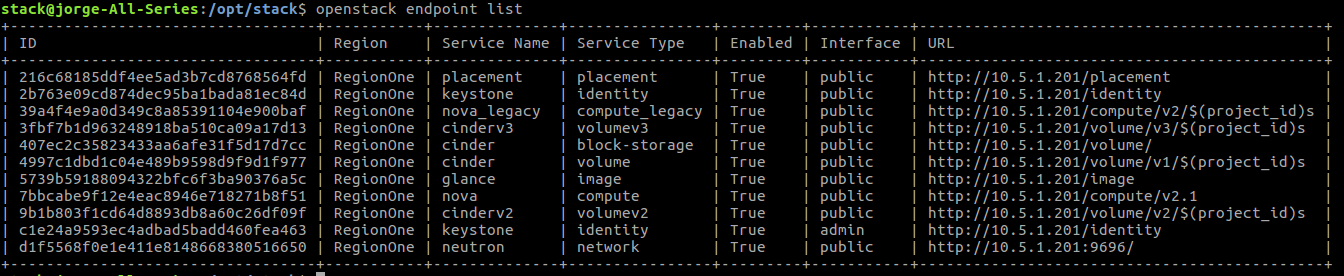
\includegraphics[width=1\textwidth]{imagenes/capitulo4/endpointlist.png}
    \caption{Lista de endpoints.}
	\vspace{0.3cm}
    \label{endpointlist}
\end{figure}

Pero aún así, esta forma de trabajo requiere trabajar con comandos complicados, motivo por el que existe Horizon. En la Fig.\ref{DashboardInicio} podemos ver el listado de los endpoints cliclando en "Acceso a la API" al acceder al escritorio o \textit{dashboard} de Horizon. Esta forma de trabajar es mucho más intuitiva al ser gráfica que el resto y será la preferida en algunos casos.


\begin{figure}
    \centering
    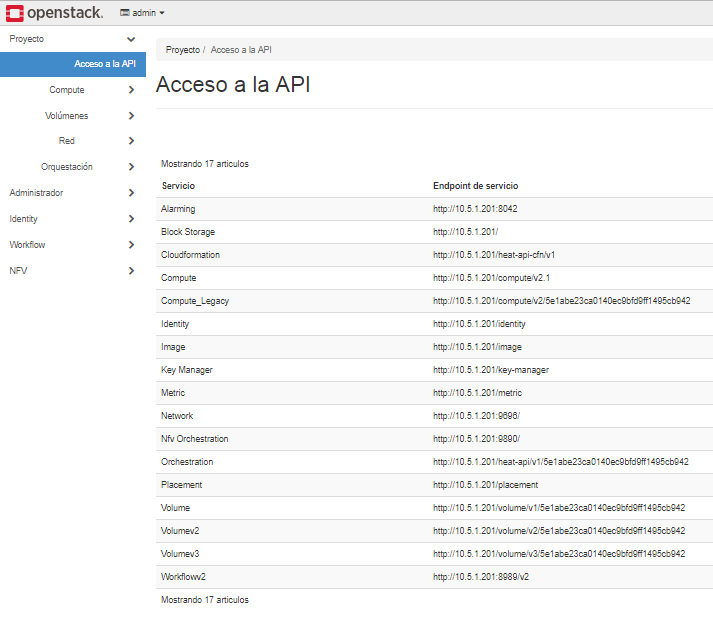
\includegraphics[width=1\textwidth]{imagenes/capitulo4/endpointlistHorizon.png}
    \caption{Lista de endpoints desde Horizon.}
	\vspace{0.3cm}
    \label{DashboardInicio}
\end{figure}

\section{Heat} \label{subchap:heat}

\begin{figure}
    \centering
    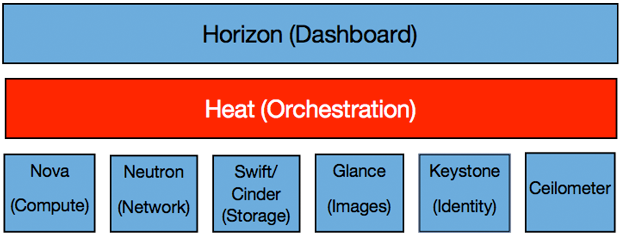
\includegraphics[width=0.7\textwidth]{imagenes/capitulo4/coordinacionHEat.png}
    \caption{Heat: capa de orquestación.}
	\vspace{0.3cm}
    \label{CapaHeat}
\end{figure}

En el capítulo \ref{chap:implementacion} donde vamos a ver como implementar nuestro entorno, veremos como utilizar el dashboard de Horizon y como trabajar desde la CLI. En los comienzos del cloud computing, aprovisionar de recursos mediante la línea de comandos pronto dejó de ser viable y los administradores comenzaron a realizar scripts en bash con la CLI para automatizar la creación de entornos. Pero pronto empezó a dar problemas este método. ¿Qué ocurre si ejecutamos un script accidentalmente, o si queremos eliminar sólo algunos recursos, o bien hacer un único cambio? Esta es la motivación del surgimiento de Heat. Además, esta evolución hacia Heat la veremos claramente tras leer el capítulo \ref{chap:implementacion} de implementación, en el que se verá la administración del entorno con estas herramientas.

Heat se introdujo en 2013 con la versión \textit{Grizzly} de OpenStack. Se basa en una pila o \textit{stack} que no es mas que una descripción de los parámetros de orquestación donde se indican todos los recursos de OpenStack a aprovisionar. Heat se ocupa por tanto del aprovisionamiento y la configuración sin necesidad de preocuparnos de las dependencias o el orden de ejecución, creando así una capa de abstracción entre los servicios básicos (Fig.\ref{CapaHeat}). Además, Heat es compatible con  el formato de plantillas de AWS CloudFormation.


\subsection{Arquitectura de Heat}
Hay cuatro componentes esenciales de un proyecto en Heat que podemos ver en la Fig.\ref{heat_architecture}, cada uno con una única función \cite{dorn_heat_2017}:
\begin{itemize}
\item \textbf{heat}. Es la CLI que se comunica con la API de heat, heat-api.
\item \textbf{heat-api}. Es el componente que proporciona una API REST nativa de OpenStack que procesa las solicitudes y las envía al motor heat-engine.
\item \textbf{heat-api-cfn}. Este componente proporciona una API de consulta del estilo AWS que es compatible con AWS CloudFormation y procesa las solicitudes y las envía a heat-engine.
\item \textbf{heat-engine}. Es el cerebro de la operación y hace el trabajo principal de orquestar el lanzamiento de plantillas o \textit{templates} y proporcionar respuesta al usuario de la API.
\end{itemize}

\begin{figure}
    \centering
    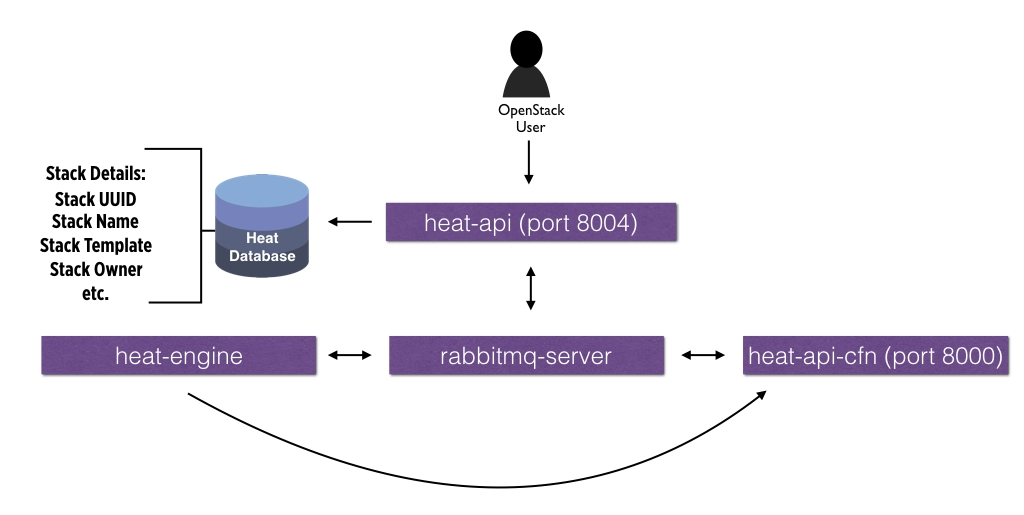
\includegraphics[width=0.7\textwidth]{imagenes/capitulo4/heat_architecture.png}
    \caption{Arquitectura de Heat.}
	\vspace{0.3cm}
    \footnotesize{Fuente: Matt Dorn, "Preparing for the Certified OpenStack Administrator Exam" Packt Publishing, 2017 }
    \label{heat_architecture}
\end{figure}


\subsection{Conceptos sobre Heat}

Ahora que conocemos los componentes de Heat vamos a presentar una serie de conceptos más sobre esta herramienta de orquestación:

\begin{itemize}
\item \textbf{Resources}. Son objetos que se crearán o modificarán durante la orquestación. Los recursos pueden ser redes, routers, subredes, instancias, volúmenes, direcciones IP flotantes, grupos de seguridad y más.
\item \textbf{Stack}. En Heat, una pila o stack es una colección de recursos.
\item \textbf{Parameters}. Permiten al usuario proporcionar información a la plantilla durante la implementación. Por ejemplo, si desea ingresar el nombre de una instancia durante la orquestación, ese nombre podría ingresarse como un parámetro en la plantilla y cambiarse cada vez que se ejecute.
\item \textbf{Template}. Plantilla en la que se indica como se define y describe un stack con código.
\item \textbf{Output}. Como su nombre indica, las salidas proporcionan información al usuario.
\end{itemize}

\subsection{Funcionamiento de Heat}
Ahora que entendemos los conceptos básicos sobre Heat, podemos comprender mejor cómo funciona.

\begin{enumerate}
\item La orquestación se define en un template al describir los objetos (recursos) en un formato legible y fácilmente entendible.
\item El usuario crea el stack que hará que la herramienta heat-cli apunte al archivo y a los parámetros de la plantilla.
\item La herramienta heat-cli se comunica con  heat-api.
\item El heat-api envía la solicitud al heat-engine.
\item El heat-engine procesa la solicitud comunicándose con las otras APIs de OpenStack y devuelve la salida al usuario.
\end{enumerate}

\subsection{Heat Orchestration Template}

\begin{figure}
    \centering
    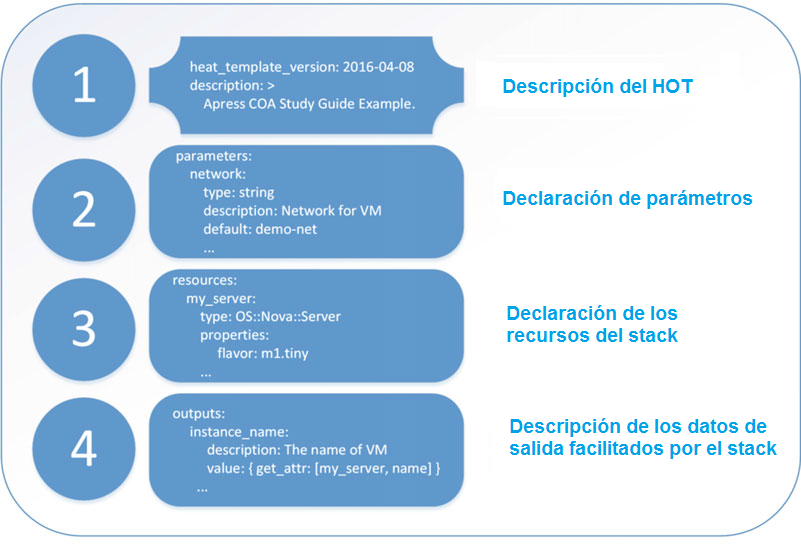
\includegraphics[width=0.7\textwidth]{imagenes/capitulo4/heat_template.png}
    \caption{Heat Orchestration Template.}
	\vspace{0.3cm}
    \footnotesize{Fuente: Andrey Markelov, “Certified OpenStack Administrator Study Guide”, apress, 2016 }
    \label{heat_template}
\end{figure}

Todos estos elementos aparecen al crear una plantilla como se aprecia en la Fig.\ref{heat_template} que muestra la anatomía de un template en Heat conocida como HOT (Heat Orchestration Template).

Una plantilla de Heat suele ser un archivo YAML, un lenguaje de serialización basado en JSON cuyo fin es su fácil comprensión y que contiene los siguientes campos \cite{dorn_horizon_2017}:

\begin{itemize}
\item Version.
\item Description.
\item Parameters.
\item Resources.
\item Output.
\end{itemize}

Sólo son obligatorios tres de los campos antes mencionados para obtener una plantilla básica: version, description y resources. 

%“” 
\section{Tacker}
Tacker es un proyecto oficial de OpenStack que construye un gestor genérico de VNF que se conoce como VNF Manager (VNFM) y un orquestador de NFV, NFV Orchestrator (NFVO), para implementar y operar con los servicios de red y las funciones de red virtual (VNF), en una plataforma que proporcione la infraestructura como OpenStack. 

Tacker se basa en ETSI MANO Architectural Framework \ref{arquitectura-NFV} para formar su arquitectura \ref{TackerArquitectura} y proporciona un stack funcional para la orquestación de servicios de red extremo a extremo utilizando VNFs.\cite{noauthor_tacker_nodate}

\begin{figure}
    \centering
    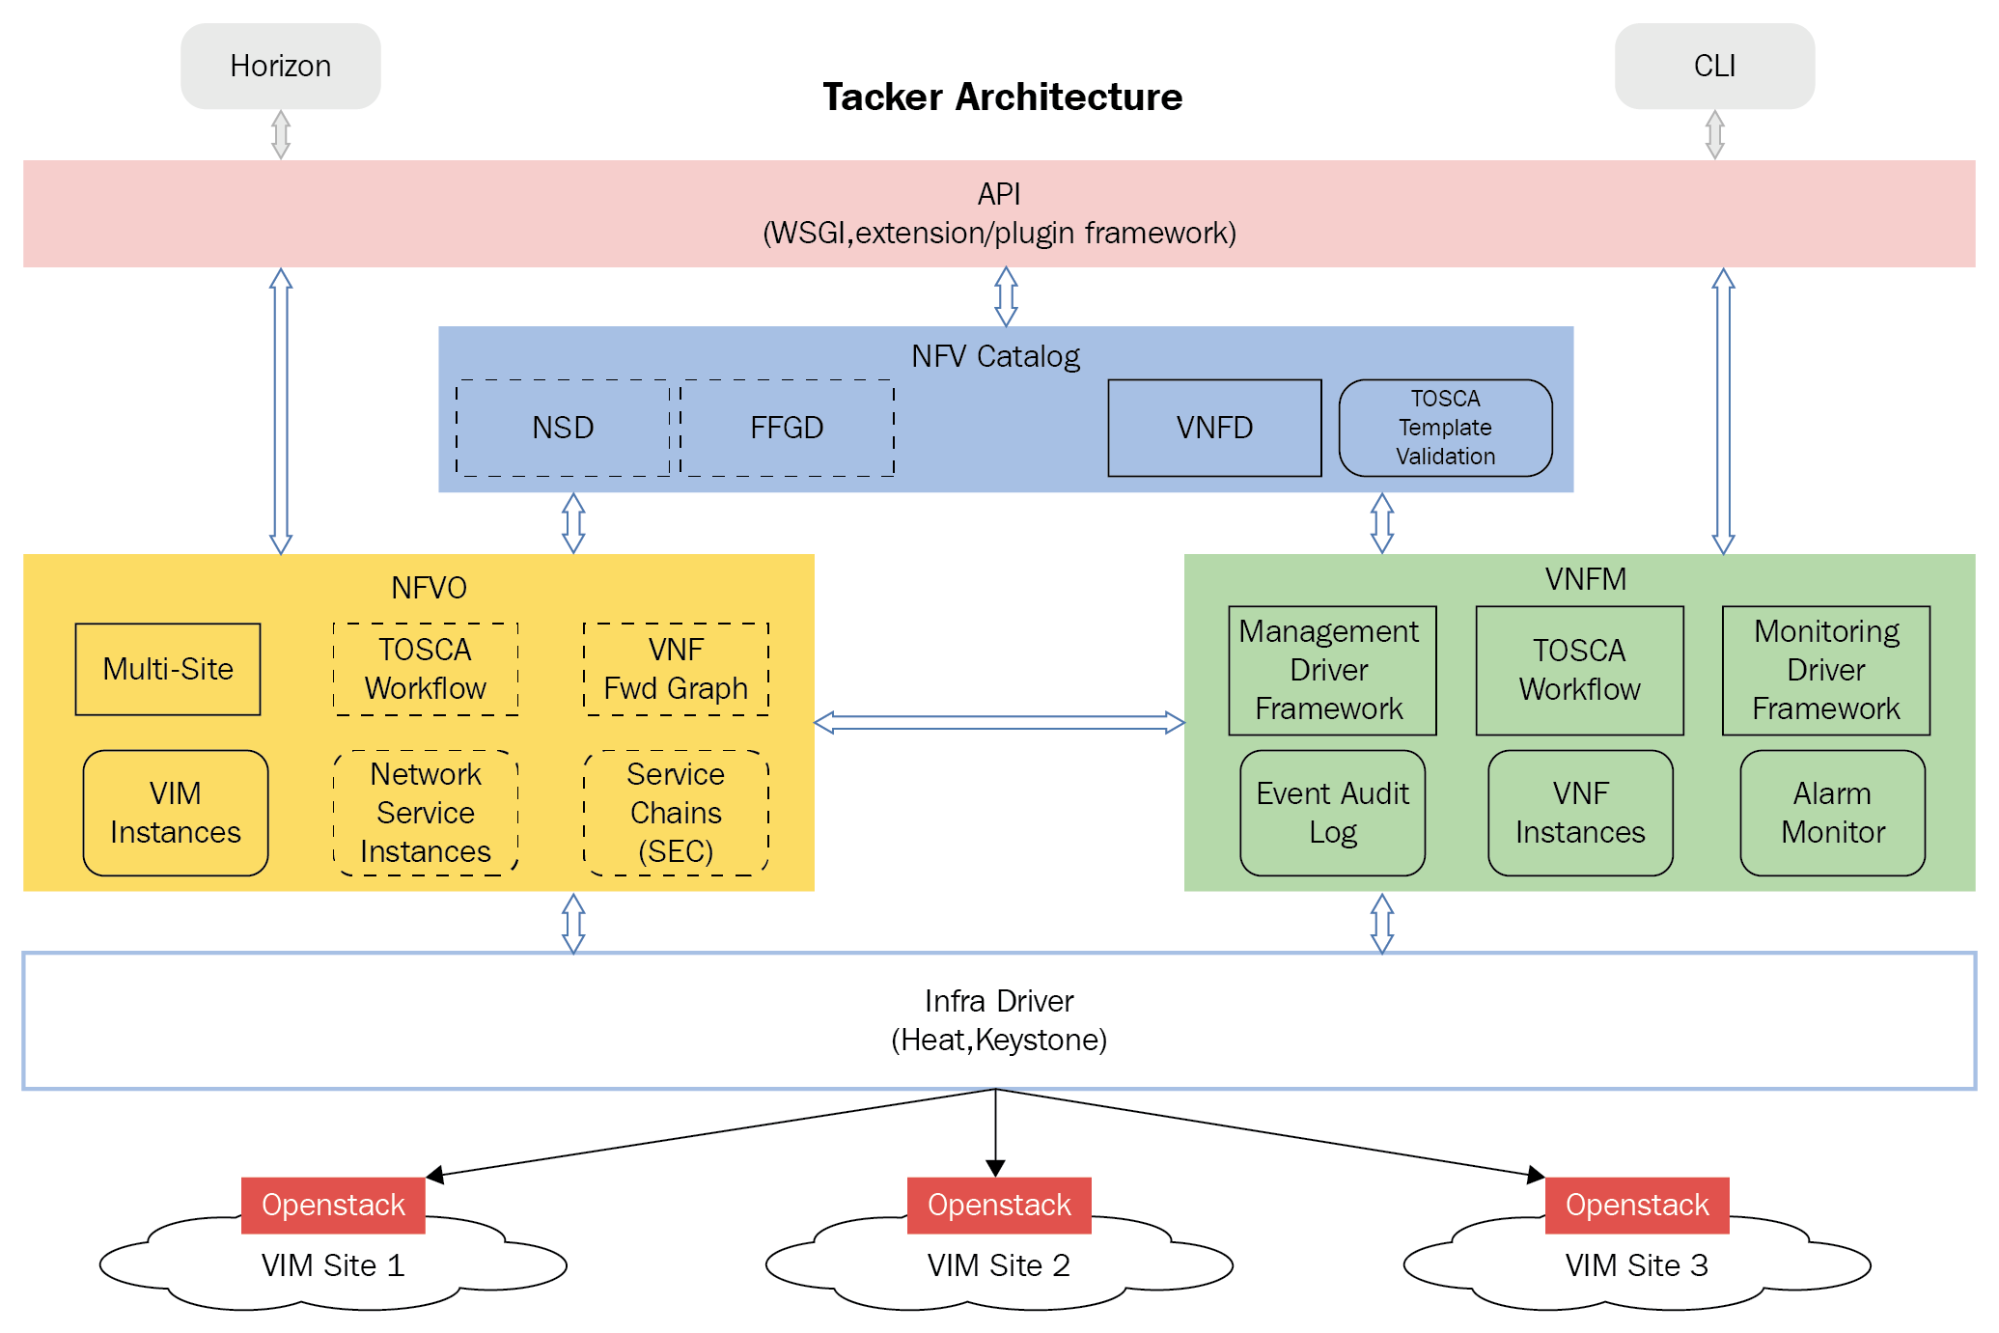
\includegraphics[width=0.7\textwidth]{imagenes/capitulo4/TackerArquitectura.png}
    \caption{Arquitectura de Tacker.}
	\vspace{0.3cm}
    \footnotesize{Fuente: Openstack Wiki}
    \label{TackerArquitectura}
\end{figure}

\begin{tcolorbox}[colback=orange!5!white,colframe=orange!75!black]
Jorge: Entiendo que lo siguiente aún no está hecho, porque habría que poner algún texto introductorio...
\end{tcolorbox}


\subsection{Motivación de Tacker}
En la mayoría de las demandas en telecomunicaciones, la alta disponibilidad y fiabilidad en su infraestructura es crítica. 

Al igual que la mayoría de las plataformas cloud y aplicaciones nativas en la nube, esto se logra a través de la escalabilidad horizontal de la arquitectura a consta de dejar a un lado las prácticas tradicionales de escalabilidad vertical en las que únicamente se requiere cada vez de más hardware y mayor capacidad. 

A pesar de no poder asegurar proporcionar el 99.999\% del tiempo de actividad del hardware en un entorno cloud, si podemos crear mecanismos que hagan que los servidores trabajen como un clúster con la finalidad de repartir el trabajo y asegurar alta disponibilidad. 

De esto trata la escalabilidad horizontal, cuya naturaleza es distribuida. Más allá de desplegar una infraestructura celular usando distintos nodos de Nova en OpenStack, Tacker ayuda a aumentar la disponibilidad. 

\subsection{Funciones de Tacker}
Dentro de los recursos y funciones de red virtual extremo a extremo que proporciona encontramos: 

\subsubsection{Catálogo NFV:} 
\begin{itemize}
\item VNF Descriptors, (VNFD).
\item Network Services Descriptors, (NSD).
\item VNF Forwarding Graph Descriptors, (VNFFGD).
\end{itemize}

Todos estos descriptores se basan OASIS TOSCA \cite{noauthor_tosca_nodate} y proporcionan algunos requisitos para definir descriptores de servicio de red (NSD), descriptores VNF (VNFD) y descriptores de gráficos de reenvío VNF (VNFFGD) utilizando \textit{TOSCA templates}. Estas plantillas se analizan y se traducen en plantillas de Heat, transmitiéndose después a un controlador que interactúa con la infraestructura de OpenStack, Heat y Keystone. La relación de estos descriptores con la arquitectura de Tacker podemos verla en la Fig.\ref{TackerArquitecturaDescriptores}.

\begin{figure}
    \centering
    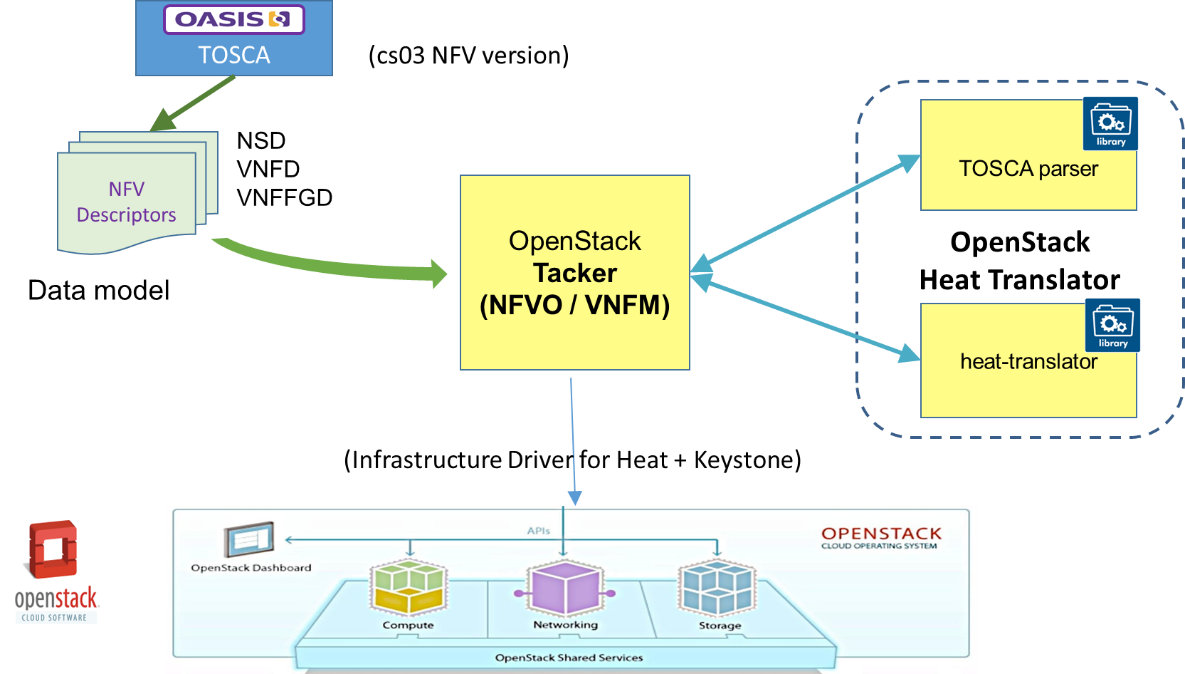
\includegraphics[width=0.7\textwidth]{imagenes/capitulo4/DescriptoresTacker.png}
    \caption{Descriptores en arquitectura de Tacker.}
	\vspace{0.3cm}
    \footnotesize{Fuente: Openstack Wiki}
    \label{TackerArquitecturaDescriptores}
\end{figure}

\subsubsection{VNFM:} 
\begin{itemize}
\item Ciclo de vida básico de una VNF (crear / actualizar / eliminar).
\item Posicionamiento mejorado basado en plataforma (EPA) de cargas de trabajo NFV de alto rendimiento.
\item Supervisión del estado de las VNFs implementadas.
\item Auto-recupearción / auto-escalado  de VNFs basado en políticas.
\item Facilitar la configuración inicial de cada VNF.
\end{itemize}

\subsubsection{NFVO:} 
\begin{itemize}
\item Implementación de servicios de red  extremo a extremo mediante el uso de plantillas que incorporan VNFs.
\item Políticas de despliegue de VNF para garantizar su formación de manera eficiente.
\item Conexión de VNFs mediante SFC (\textit{Service Function Chaining}),  especificadas en un descriptor VNF Forwarding Graph Descriptor.
\item Verificaciones de recursos VIM y asignación de recursos.
\item Capacidad de organizar VNFs en múltiples VIM y regiones múltiples (POPs).
\end{itemize}

\section{Ceilometer}
Dentro de los servicios de telemetría que ofrece OpenStack encontramos \textit{Ceilometer}. El proyecto Ceilometer es un servicio de recopilación de datos de medición y eventos de los servicios de OpenStack. Estos datos pueden ser utilizados por otros proyectos de OpenStack para actuar en función de ellos como en el caso de Heat y son almancenados en una base de datos \textit{MongoDB}.

El servicio de telemetría consta de los siguientes componentes \cite{noauthor_celiometer_nodate}:

\begin{itemize}
\item \textbf{Compute agent (ceilometer-agent-compute)}. Se ejecuta en cada nodo de cómputo para sondeos y estadísticas de utilización de recursos.
\item \textbf{Central agent (ceilometer-agent-central)}. Se ejecuta en un servidor de administración central para sondear las estadísticas de utilización de recursos no vinculados a instancias o nodos de cómputo. Se pueden iniciar múltiples agentes para escalar el servicio horizontalmente. 
\item\textbf{Notification agent (ceilometer-agent-notification)}. Se ejecuta en un servidor central de administración y consume mensajes de la o las colas de mensajes para generar datos de eventos y medición. Los datos se entregan a los destinatarios pertinentes.
\end{itemize}




